\documentclass[article, 1.5space, letterpaper, 12pt, oneside, header, footer]{SydeClass}
\graphicspath{{images/}}
\usepackage{subfigure}
\usepackage{eqnarray}


% --------- Title Info -----------
\titlestyle{design} % used in SydeTitle.tex. Can equal one of the following values: design, work

\title{Lab 1}
\subtitle{Fundamentals of Image Processing}

\coursecode{SYDE 475}
\department{Systems Design Engineering}

\author{Colin Heics, 20240543}
\authorheader{C. Heics}
\authortwo{Neil Sokol, 20265064}
\authorheadertwo{N. Sokol}

\date{\today}
\instructor{Alex Wong}

\subsectionfont{\normalsize}
\setcounter{secnumdepth}{2}
\setcounter{tocdepth}{1}

\usepackage{listings}
\usepackage{color}
\usepackage{textcomp}
\definecolor{listinggray}{gray}{0.9}
\definecolor{lbcolor}{rgb}{0.9,0.9,0.9}
\lstset{
	backgroundcolor=\color{lbcolor},
	tabsize=4,
	rulecolor=,
	language=matlab,
        basicstyle=\scriptsize,
        upquote=true,
        aboveskip={1.5\baselineskip},
        columns=fixed,
        showstringspaces=false,
        extendedchars=true,
        breaklines=true,
        prebreak = \raisebox{0ex}[0ex][0ex]{\ensuremath{\hookleftarrow}},
        frame=single,
        showtabs=false,
        showspaces=false,
        showstringspaces=false,
        identifierstyle=\ttfamily,
        keywordstyle=\color[rgb]{0,0,1},
        commentstyle=\color[rgb]{0.133,0.545,0.133},
        stringstyle=\color[rgb]{0.627,0.126,0.941},
}

% ############  ############
\begin{document}

% ---------- Title ------------

%% Use the command "
%% Use the command "
%% Use the command "\input{SydeTitle}" in your main file to include this file.

\begin{titlepage}
	\makeatletter % use .cls usage for <at>
	
	\pagestyle{empty}
	\equalmargins
	
	\ifthenelse{\equal{\@titlestyle}{work}}{
		\begin{center}
			\vspace*{2em}

			University of Waterloo\\
			Faculty of Engineering\\
			Department of Systems Design Engineering

			\null\vfill
		
			\Huge\@title \\
			\ifdefined \@subtitle \Large\@subtitle \\ \fi
			\normalsize

			\null\vfill
		
			\@company\\
			\@companyaddress \vspace{2em}
		
			\@author\\
			\@date
		\end{center}
	}{\relax} % end if
	
	\ifthenelse{\equal{\@titlestyle}{design}}{
		\begin{center}
			\vspace*{5em}
	
			\Huge\@title \\
			\ifdefined \@subtitle \Large\@subtitle \\ \fi
			\normalsize
	
			\vfill
		
			A Report Submitted in Partial Fulfilment\\
			of the Requirements for \@coursecode \vspace{4em}
		
			\ifdefined \@groupname \@groupname \\ \fi
		  \@author \\
			\ifdefined \@authortwo \@authortwo \\ \fi
			\ifdefined \@authorthree \@authorthree \\ \fi
			\ifdefined \@authorfour \@authorfour \\ \fi
		  \vspace{3em}
		
			Faculty of Engineering \\
			\ifdefined \@department Department of \@department \\ \fi
			\vspace{3em}
		
			\@date \\
			
			\ifdefined \@instructor Course Instructor: \@instructor \\ \fi
			\ifdefined \@supervisor Project Supervisor: \@supervisor \\ \fi
			
		\end{center}
	}{\relax} % end if
	
	\makeatother % return to document usage for <at>
\end{titlepage}

%\pagestyle{plain}
%\offsetmargins" in your main file to include this file.

\begin{titlepage}
	\makeatletter % use .cls usage for <at>
	
	\pagestyle{empty}
	\equalmargins
	
	\ifthenelse{\equal{\@titlestyle}{work}}{
		\begin{center}
			\vspace*{2em}

			University of Waterloo\\
			Faculty of Engineering\\
			Department of Systems Design Engineering

			\null\vfill
		
			\Huge\@title \\
			\ifdefined \@subtitle \Large\@subtitle \\ \fi
			\normalsize

			\null\vfill
		
			\@company\\
			\@companyaddress \vspace{2em}
		
			\@author\\
			\@date
		\end{center}
	}{\relax} % end if
	
	\ifthenelse{\equal{\@titlestyle}{design}}{
		\begin{center}
			\vspace*{5em}
	
			\Huge\@title \\
			\ifdefined \@subtitle \Large\@subtitle \\ \fi
			\normalsize
	
			\vfill
		
			A Report Submitted in Partial Fulfilment\\
			of the Requirements for \@coursecode \vspace{4em}
		
			\ifdefined \@groupname \@groupname \\ \fi
		  \@author \\
			\ifdefined \@authortwo \@authortwo \\ \fi
			\ifdefined \@authorthree \@authorthree \\ \fi
			\ifdefined \@authorfour \@authorfour \\ \fi
		  \vspace{3em}
		
			Faculty of Engineering \\
			\ifdefined \@department Department of \@department \\ \fi
			\vspace{3em}
		
			\@date \\
			
			\ifdefined \@instructor Course Instructor: \@instructor \\ \fi
			\ifdefined \@supervisor Project Supervisor: \@supervisor \\ \fi
			
		\end{center}
	}{\relax} % end if
	
	\makeatother % return to document usage for <at>
\end{titlepage}

%\pagestyle{plain}
%\offsetmargins" in your main file to include this file.

\begin{titlepage}
	\makeatletter % use .cls usage for <at>
	
	\pagestyle{empty}
	\equalmargins
	
	\ifthenelse{\equal{\@titlestyle}{work}}{
		\begin{center}
			\vspace*{2em}

			University of Waterloo\\
			Faculty of Engineering\\
			Department of Systems Design Engineering

			\null\vfill
		
			\Huge\@title \\
			\ifdefined \@subtitle \Large\@subtitle \\ \fi
			\normalsize

			\null\vfill
		
			\@company\\
			\@companyaddress \vspace{2em}
		
			\@author\\
			\@date
		\end{center}
	}{\relax} % end if
	
	\ifthenelse{\equal{\@titlestyle}{design}}{
		\begin{center}
			\vspace*{5em}
	
			\Huge\@title \\
			\ifdefined \@subtitle \Large\@subtitle \\ \fi
			\normalsize
	
			\vfill
		
			A Report Submitted in Partial Fulfilment\\
			of the Requirements for \@coursecode \vspace{4em}
		
			\ifdefined \@groupname \@groupname \\ \fi
		  \@author \\
			\ifdefined \@authortwo \@authortwo \\ \fi
			\ifdefined \@authorthree \@authorthree \\ \fi
			\ifdefined \@authorfour \@authorfour \\ \fi
		  \vspace{3em}
		
			Faculty of Engineering \\
			\ifdefined \@department Department of \@department \\ \fi
			\vspace{3em}
		
			\@date \\
			
			\ifdefined \@instructor Course Instructor: \@instructor \\ \fi
			\ifdefined \@supervisor Project Supervisor: \@supervisor \\ \fi
			
		\end{center}
	}{\relax} % end if
	
	\makeatother % return to document usage for <at>
\end{titlepage}

%\pagestyle{plain}
%\offsetmargins

% ############ Chapters ############
\pagenumbering{arabic}

\section{Noise Generation}

When evaluating image processing algorithms, it is important to see how they perform under various levels of noise.


\begin{figure}[ht]
\centering
	\subfigure[Original image]{
	
\includegraphics[width=0.45\linewidth]{question2/toy}
	}
\end{figure}

\begin{figure}[ht]
\centering
	\subfigure[Image with Gaussian Noise]{
	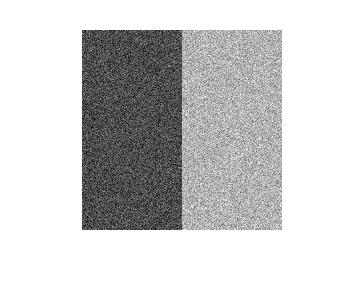
\includegraphics[width=0.45\linewidth]{question2/gauss}
	}
	\subfigure[Histogram of Gaussian Noise Image]{
	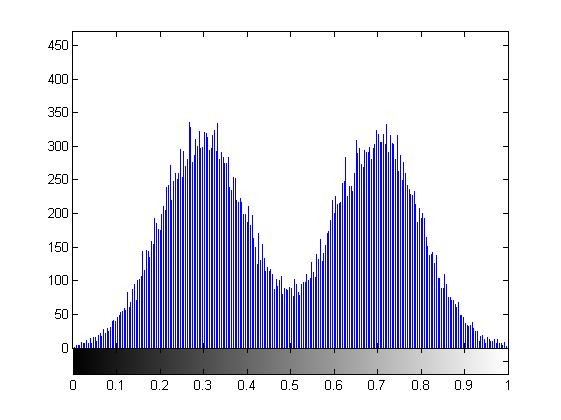
\includegraphics[width=0.45\linewidth]{question2/gauss_hist}
	}
	\subfigure[Image with Speckle Noise]{
	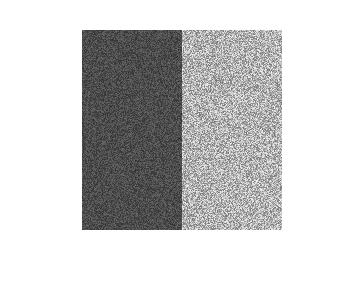
\includegraphics[width=0.45\linewidth]{question2/speckle}
	}
	\subfigure[Histogram of Speckle Noise Image]{
	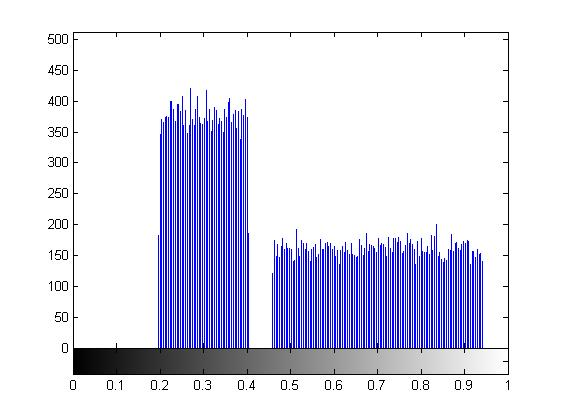
\includegraphics[width=0.45\linewidth]{question2/speckle_hist}
	}
	\subfigure[Image with Salt and Pepper]{
	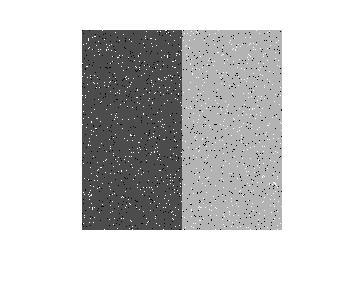
\includegraphics[width=0.45\linewidth]{question2/salt}
	}
	\subfigure[Histogram of Salt and Pepper Image]{
	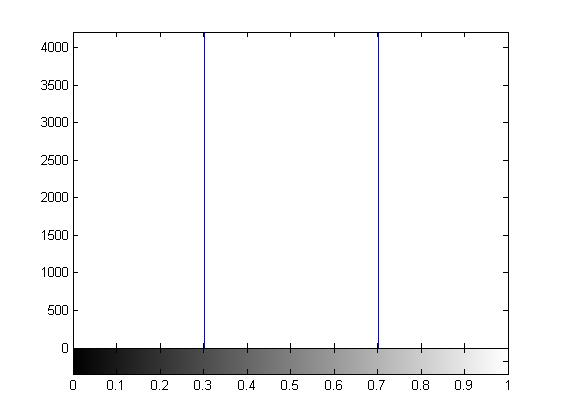
\includegraphics[width=0.45\linewidth]{question2/salt_hist}
	}
	\caption{Toy image with Gaussian, Salt and Pepper, and Speckle Noise}
	\label{fig:noiseGeneration.toy}
\end{figure}
 

\subsection{Discussion questions}

\subsubsection{ Describe each of the histograms in the context of the corresponding noise models. Why do they appear
that way?}
In the gaussian histogram, image intensities are grouped in gaussian distributions centered around the two intesity values of the original image. It appears the way it is because as additive noise, all that is being done is the gaussian distribution is added to the image. Speckled noise, which is multiplicative, appears to be a flat distribution centered around the original intensities. There is more variance around the higher original intesity value, which is due to the multiplicative nature of speckle noise.

\subsubsection{Are there visual differences between the noise contaminated images? What are they? Why}
There are some visual differences. The gaussian has a lot more extra bright or extra dark pixels, while speckled has more that are more off by a smaller intensity. This is because the gaussian is additive noise, and the speckled is multiplicative.

\subsubsection{In the speckle noise case, what is the underlying distribution used? Can you tell from the histogram?
How?}
The underlying distribution is uniform. You can tell from the histogram because the intensities are distributed roughly evenly (i.e. same number of pixels). 

\subsubsection{In the speckle noise case, you will notice that the peaks of the histogram are no longer of the same
height as they were in the original image. Also, the spread around each of the peaks is also different
from each other. Why? Hint: Noise is multiplicative}
Since the noise is multiplicative, it is proportional to the local grey level in the image. i.e. there will be a wider spread of values around higher grey levels, as we can see with the right-most spread having a higher variance.



\section{Noise Reduction in the Spatial Domain}

\clearpage
\subsection{Section0}
\begin{figure}[ht]
\centering
	\subfigure[Original image]{
	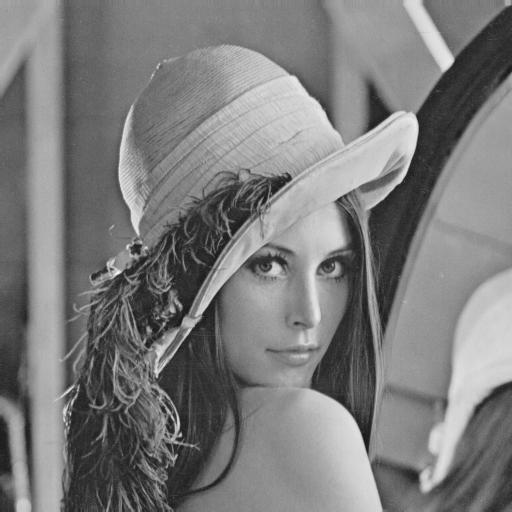
\includegraphics[width=0.45\linewidth]{question3/0_lenaBase}
	}
	\subfigure[Histogram]{
	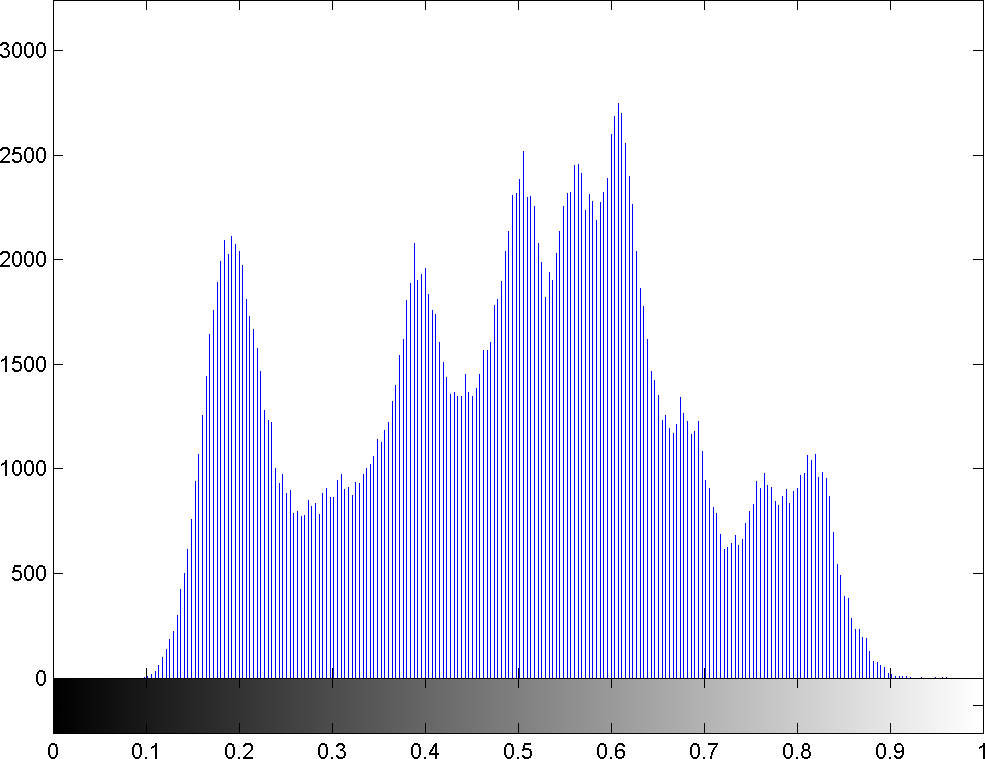
\includegraphics[width=0.45\linewidth]{question3/0_lenaBase_hist}
	}
	\subfigure[Image with gaussian noise $\mu$=0, $\sigma$=0.002; PSNR +26.99dB]{
	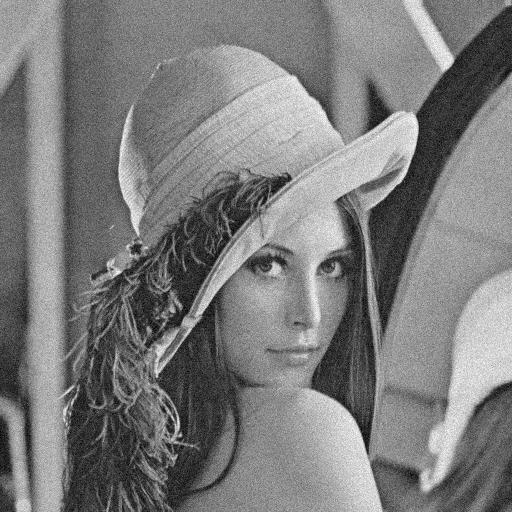
\includegraphics[width=0.45\linewidth]{question3/0_lenaNoisyGauss}
	}
	\subfigure[Histogram]{
	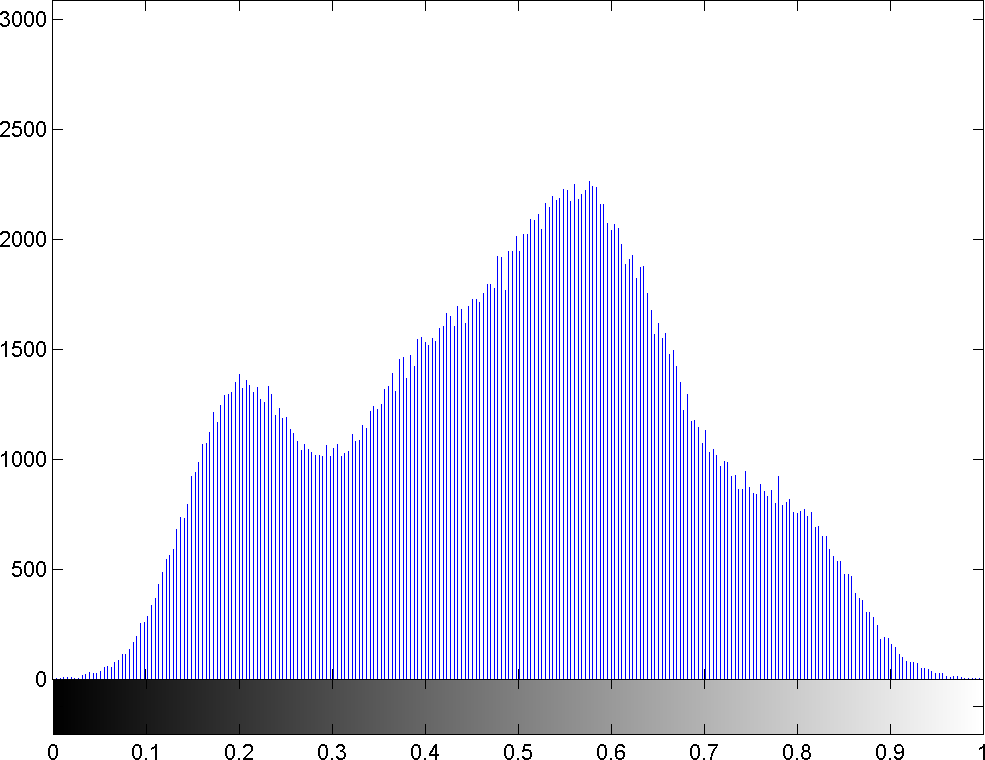
\includegraphics[width=0.45\linewidth]{question3/0_lenaNoisyGauss_hist}
	}
	\caption{Images with gaussian noise}
	\label{fig:gaussianNoise}
\end{figure}


\clearpage
\subsection{Section1}
\begin{figure}[ht]
\centering
	\subfigure[Denoised image with 3x3 average kernel; PSNR +18.42dB]{
	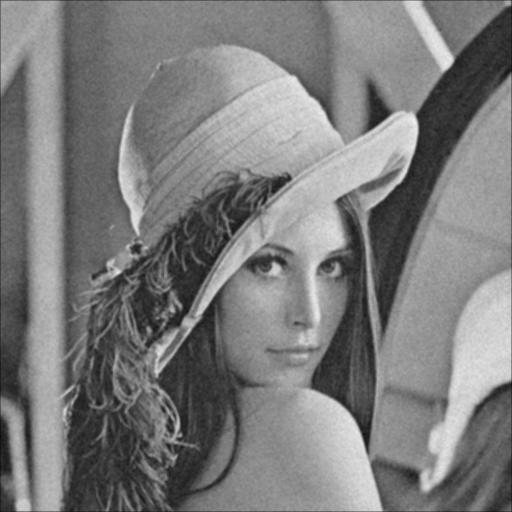
\includegraphics[width=0.45\linewidth]{question3/1_lenaDeNoisyGauss3x3avg}
	}
	\subfigure[Histogram]{
	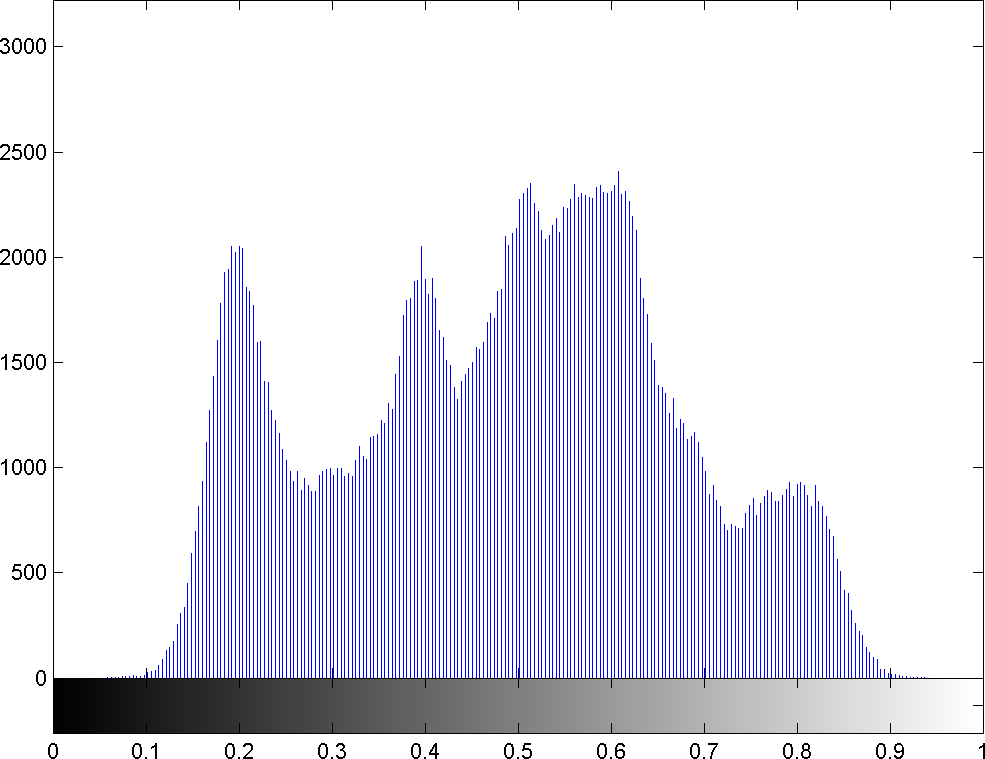
\includegraphics[width=0.45\linewidth]{question3/1_lenaDeNoisyGauss3x3avg_hist}
	}
	
	\caption{Images with gaussian noise}
	\label{fig:gaussianNoise}
\end{figure}

\clearpage
\subsection{Section2}
\begin{figure}[ht]
\centering
	\subfigure[Denoised image with 7x7 average kernel; PSNR +25.52dB]{
	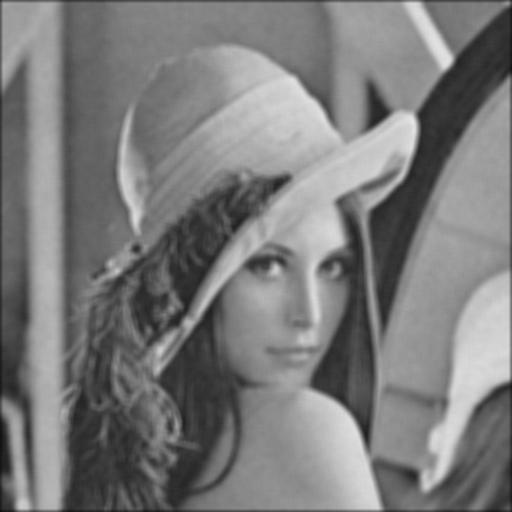
\includegraphics[width=0.45\linewidth]{question3/2_lenaDeNoisyGauss7x7avg}
	}
	\subfigure[Histogram]{
	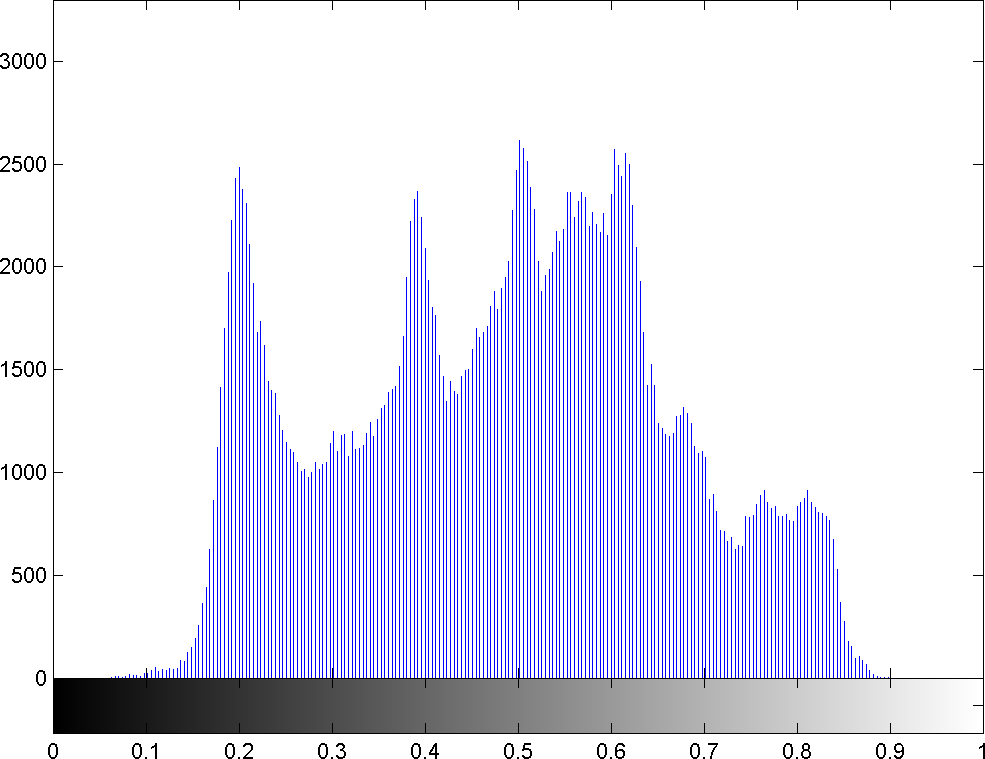
\includegraphics[width=0.45\linewidth]{question3/2_lenaDeNoisyGauss7x7avg_hist}
	}
	
	\caption{Images with gaussian noise}
	\label{fig:gaussianNoise}
\end{figure}

\clearpage
\subsection{Section3}
\begin{figure}[ht]
\centering
	\subfigure[Denoised image with 7x7 gaussian kernel; PSNR +27.08dB]{
	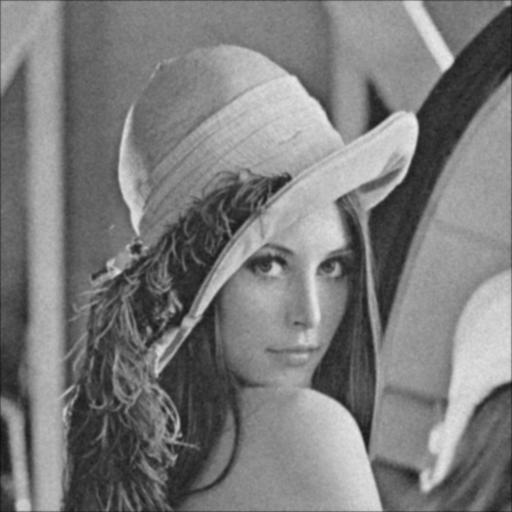
\includegraphics[width=0.45\linewidth]{question3/3_lenaDeNoisyGauss7x7avgGauss}
	}
	\subfigure[Histogram]{
	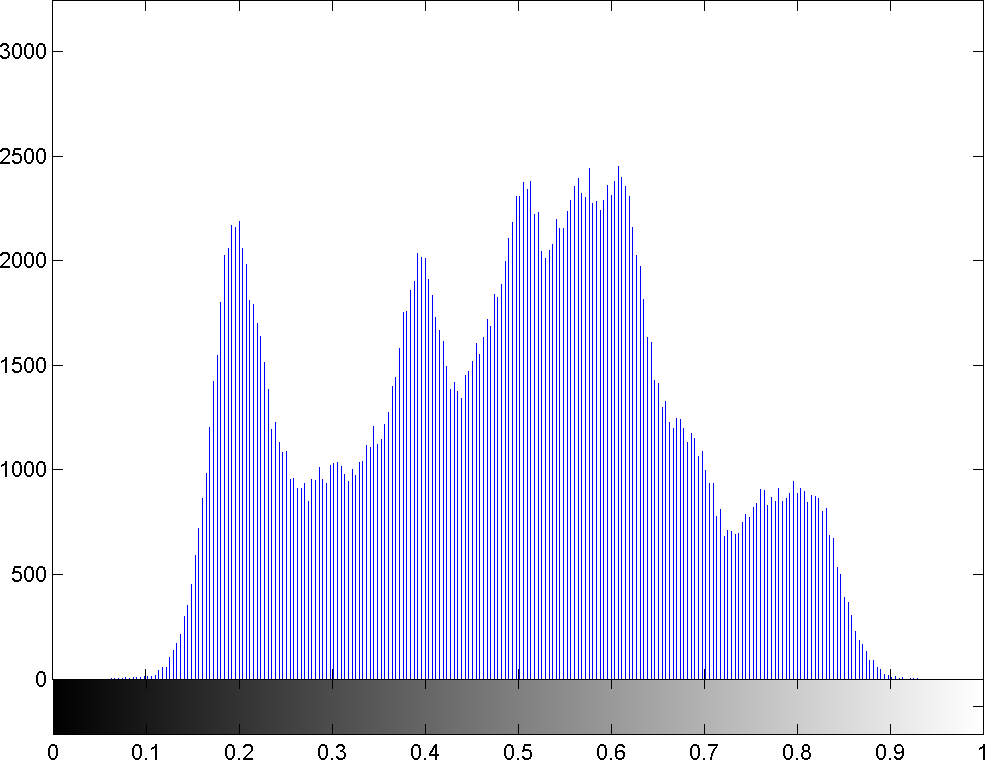
\includegraphics[width=0.45\linewidth]{question3/3_lenaDeNoisyGauss7x7avgGauss_hist}
	}
	
	\caption{Images with gaussian noise}
	\label{fig:gaussianNoise}
\end{figure}


\clearpage
\subsection{Section4}

\begin{figure}[ht]
\centering
	\subfigure[S\&P noise on original image; PSNR +18.41dB]{
	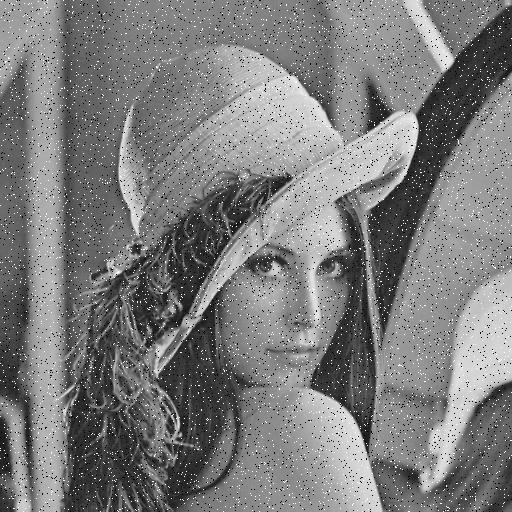
\includegraphics[width=0.45\linewidth]{question3/4_lenaNoisySp}
	}
	\subfigure[Histogram]{
	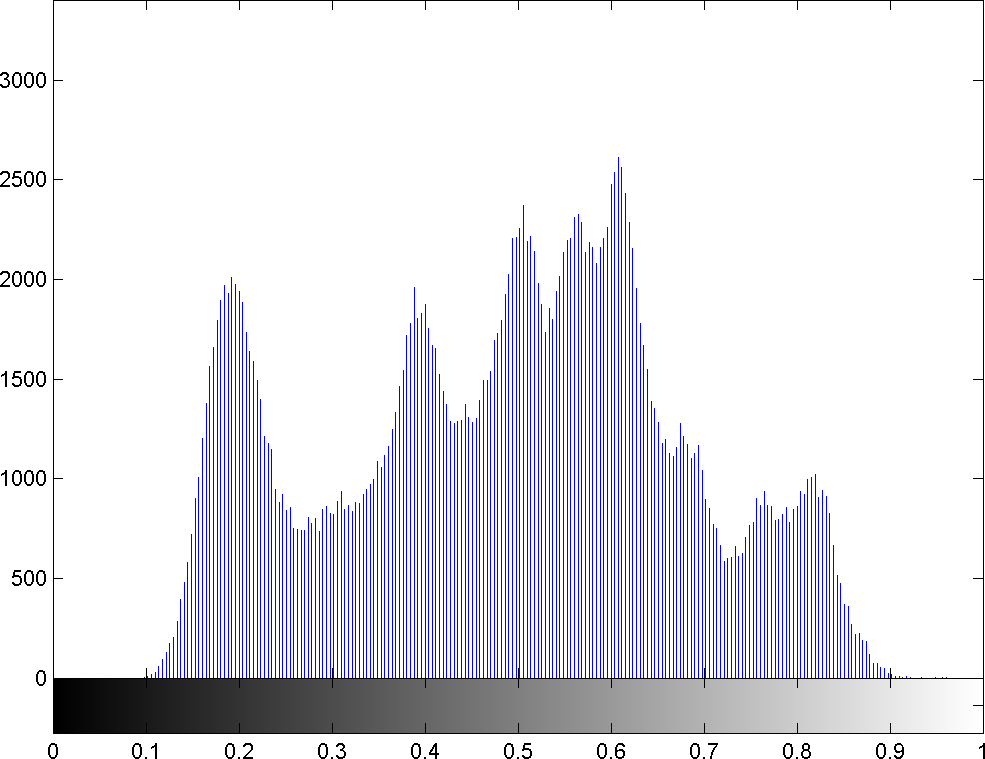
\includegraphics[width=0.45\linewidth]{question3/4_lenaNoisySp_hist}
	}
\end{figure}

\begin{figure}[ht]
\centering	
	\subfigure[S\&P denoised with 7x7 average kernel; PSNR +25.52dB]{
	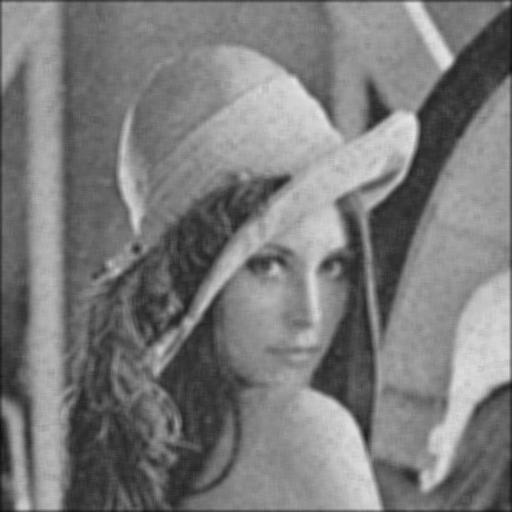
\includegraphics[width=0.45\linewidth]{question3/4_lenaDeNoisySp_7x7Avg}
	}
	\subfigure[Histogram]{
	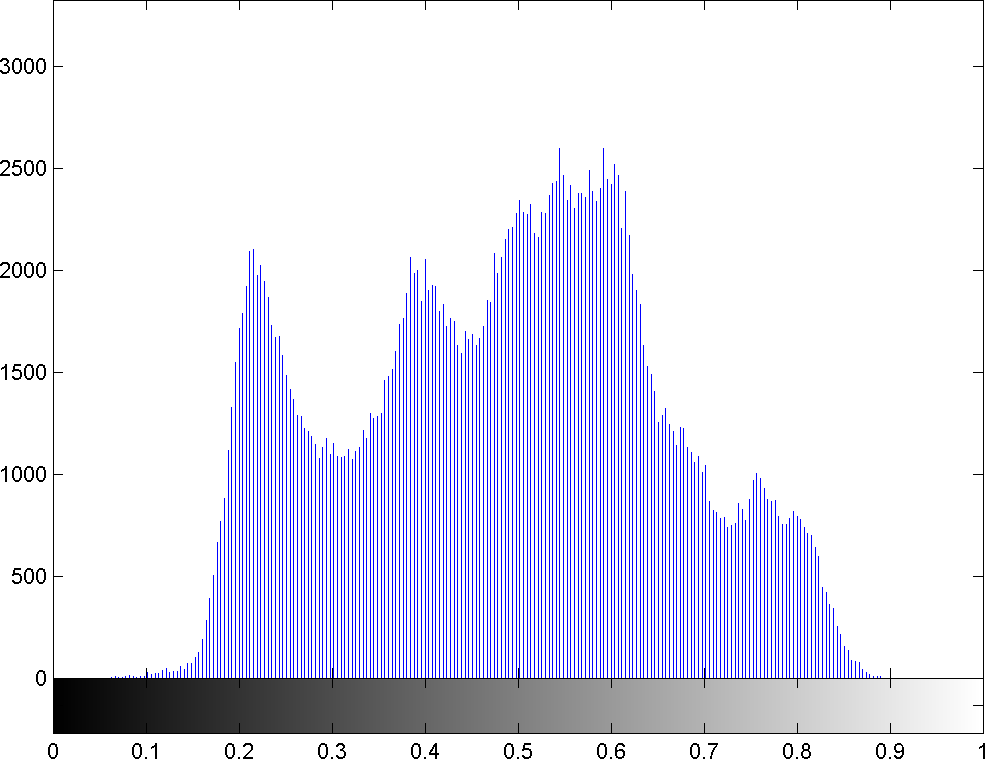
\includegraphics[width=0.45\linewidth]{question3/4_lenaDeNoisySp_7x7Avg_hist}
	}
\end{figure}

\begin{figure}[ht]
\centering
	\subfigure[S\&P denoised with 7x7 gaussian kernel; PSNR +27.08dB]{
	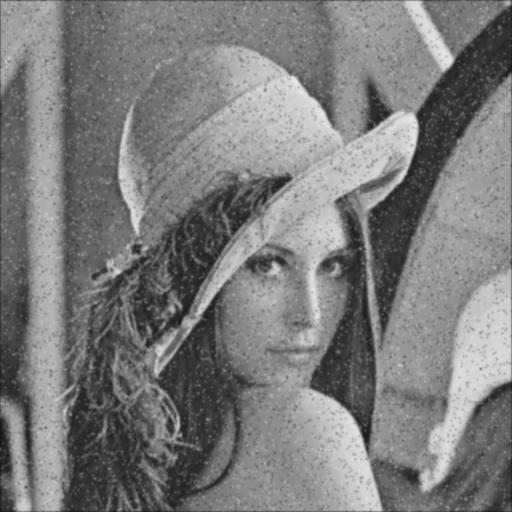
\includegraphics[width=0.45\linewidth]{question3/4_lenaDeNoisySp_7x7AvgGauss}
	}
	\subfigure[Histogram]{
	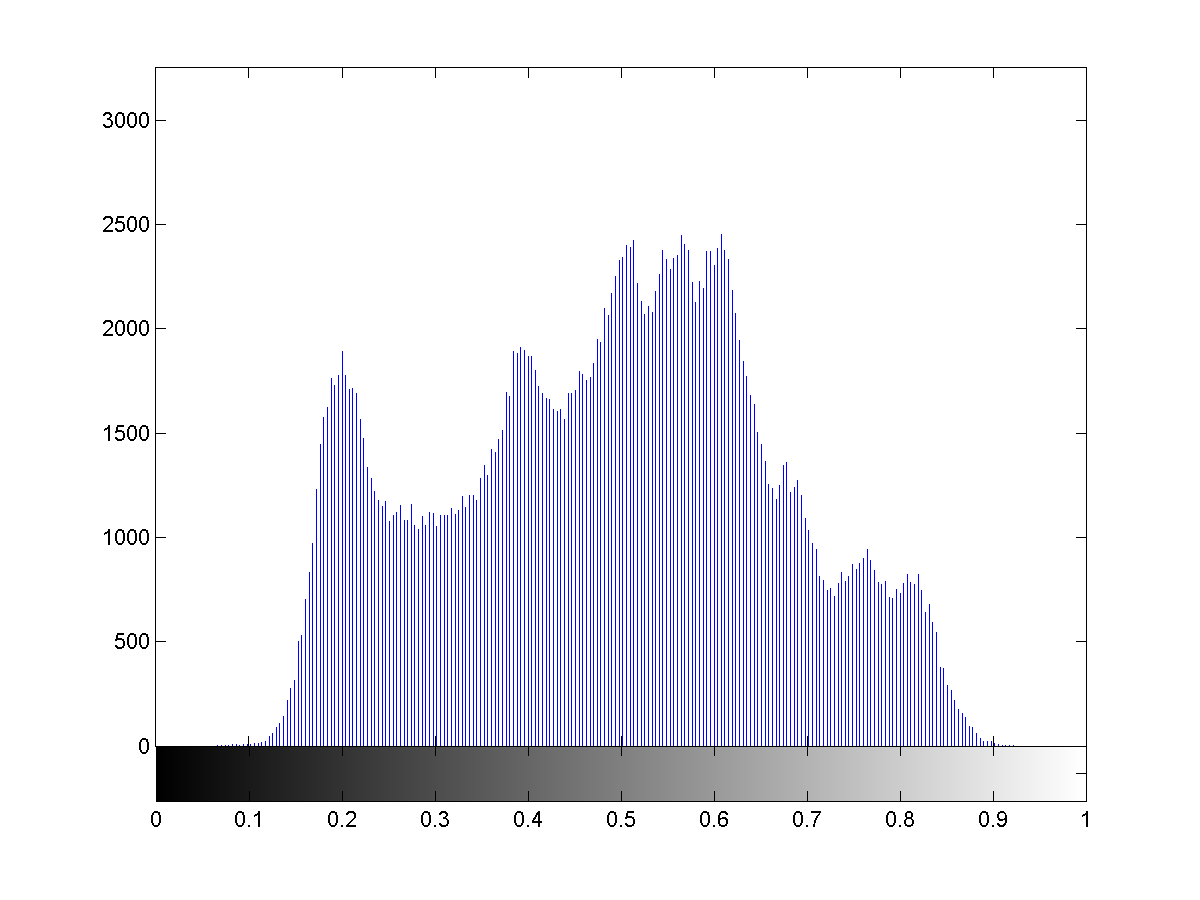
\includegraphics[width=0.45\linewidth]{question3/4_lenaDeNoisySp_7x7AvgGauss_hist}
	}
\end{figure}


\clearpage
\subsection{Section5}

\begin{figure}[ht]
\centering
	\subfigure[S\&P denoised with median filter; PSNR +34.47]{
	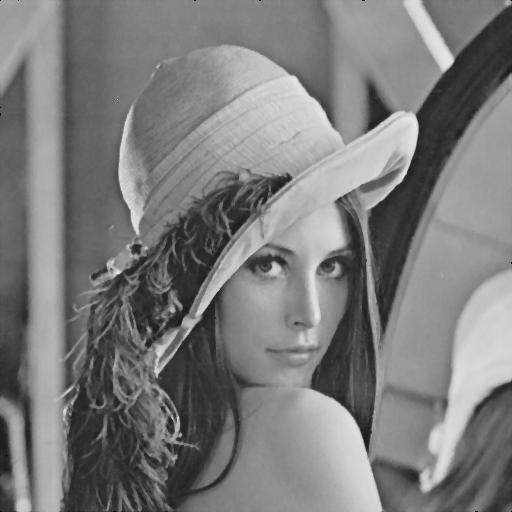
\includegraphics[width=0.45\linewidth]{question3/5_lenaDeNoisyMedian}
	}
	\subfigure[Histogram]{
	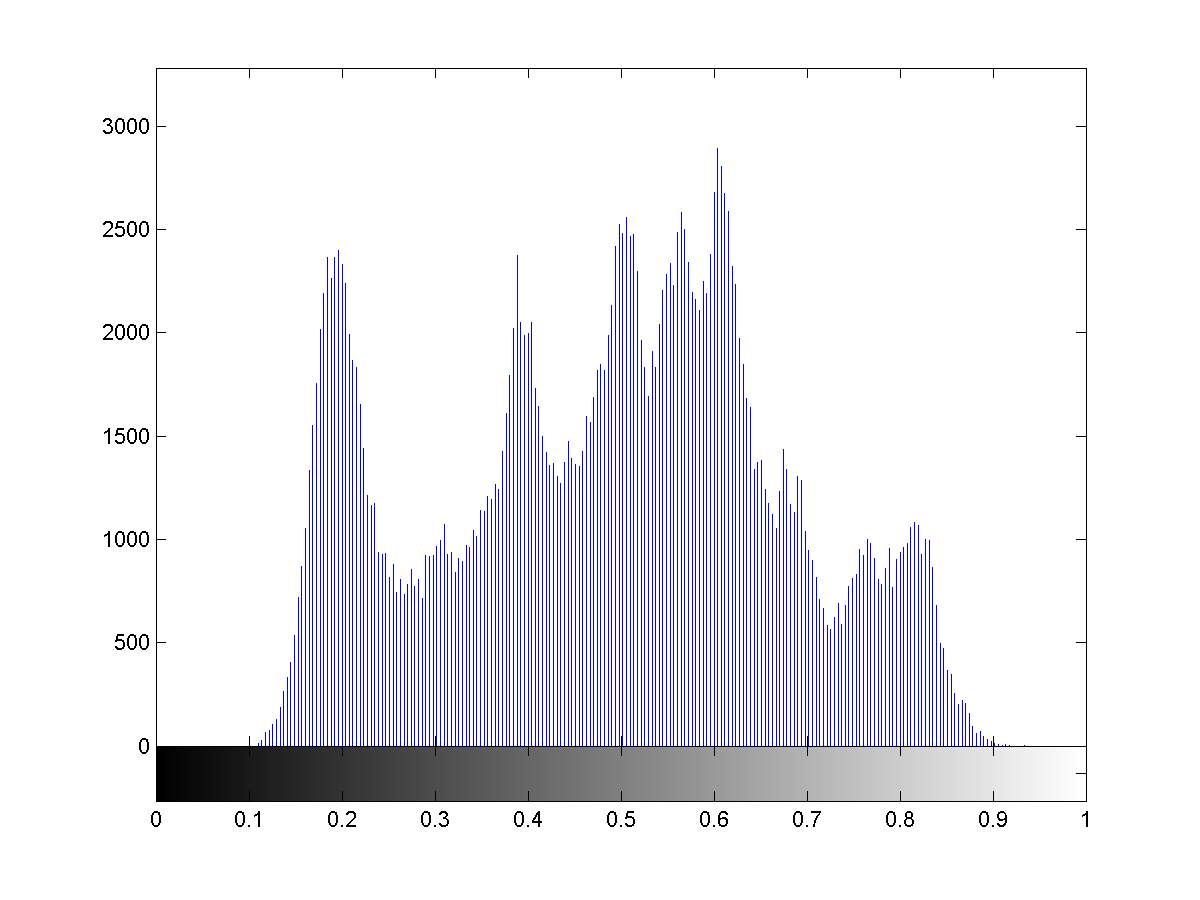
\includegraphics[width=0.45\linewidth]{question3/5_lenaDeNoisyMedian_hist}
	}
\end{figure}

\clearpage


\subsection{Discussion questions}

\subsubsection{Compare the visual difference between the noisy image and the denoised image. How well did it
work? Why? Did the PSNR decrease}


\section{Sharpening in the spatial domain}

\subsection{Section1}
\begin{figure}[ht]
\centering
	\subfigure[Base Cameraman image]{
	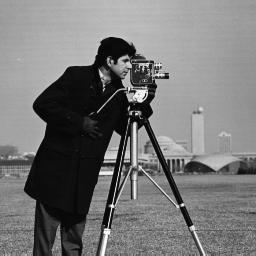
\includegraphics[width=0.45\linewidth]{question4/1_camBase}
	}
	\subfigure[Original image - Blurred image]{
	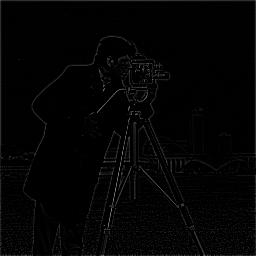
\includegraphics[width=0.45\linewidth]{question4/1_cam_highBoost}
	}
\end{figure}

\subsection{Section2}
\begin{figure}[ht]
\centering
	\subfigure[Highboosted image, A=1.0]{
	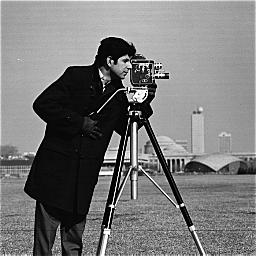
\includegraphics[width=0.45\linewidth]{question4/2_cam_highBoost_10}
	}
\end{figure}


\subsection{Section3}
\begin{figure}[ht]
\centering
	\subfigure[Highboosted image, A=0.5]{
	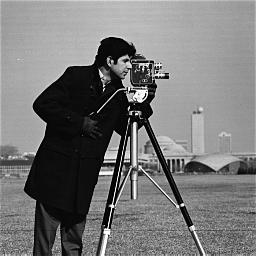
\includegraphics[width=0.45\linewidth]{question4/3_cam_highBoost_05}
	}
\end{figure}

\begin{figure}[ht]
\centering
	\subfigure[Highboosted image, A=1.5]{
	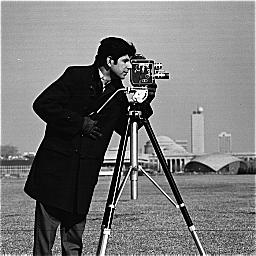
\includegraphics[width=0.45\linewidth]{question4/3_cam_highBoost_15}
	}
	\subfigure[Highboosted image, A=4.0]{
	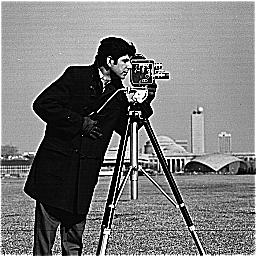
\includegraphics[width=0.45\linewidth]{question4/3_cam_highBoost_40}
	}
\end{figure}

\appendix
\newpage

% -------- Bibliography --------
%\addcontentsline{toc}{chapter}{\hspace{13pt} References}
\bibliography{refs}

\end{document}  